\documentclass{article} % For LaTeX2e
\usepackage{nips14submit_e,times}
\usepackage{amsmath}
\usepackage{amsthm}
\usepackage{amssymb}
\usepackage{mathtools}
\usepackage{hyperref}
\usepackage{url}
\usepackage{algorithm}
\usepackage[noend]{algpseudocode}
%\documentstyle[nips14submit_09,times,art10]{article} % For LaTeX 2.09

\usepackage{bbm}
\usepackage{graphicx}
\usepackage{caption}
\usepackage{subcaption}
\usepackage{MnSymbol}

\def\eQb#1\eQe{\begin{eqnarray*}#1\end{eqnarray*}}
\def\eQnb#1\eQne{\begin{eqnarray}#1\end{eqnarray}}
\providecommand{\e}[1]{\ensuremath{\times 10^{#1}}}
\providecommand{\pb}[0]{\pagebreak}
\DeclarePairedDelimiter\ceil{\lceil}{\rceil}
\DeclarePairedDelimiter\floor{\lfloor}{\rfloor}

\newcommand{\E}{\mathrm{E}}
\newcommand{\Var}{\mathrm{Var}}
\newcommand{\Cov}{\mathrm{Cov}}
\newcommand\eqD{\stackrel{\mathclap{\normalfont\mbox{d}}}{=}}

\def\Qb#1\Qe{\begin{question}#1\end{question}}
\def\Sb#1\Se{\begin{solution}#1\end{solution}}

\newenvironment{claim}[1]{\par\noindent\underline{Claim:}\space#1}{}
\newtheoremstyle{quest}{\topsep}{\topsep}{}{}{\bfseries}{}{ }{\thmname{#1}\thmnote{ #3}.}
\theoremstyle{quest}
\newtheorem*{definition}{Definition}
\newtheorem*{theorem}{Theorem}
\newtheorem*{lemma}{Lemma}
\newtheorem*{question}{Question}
\newtheorem*{preposition}{Preposition}
\newtheorem*{exercise}{Exercise}
\newtheorem*{challengeproblem}{Challenge Problem}
\newtheorem*{solution}{Solution}
\newtheorem*{remark}{Remark}
\usepackage{verbatimbox}
\usepackage{listings}
\usepackage{mathrsfs}
\title{ProbLimI: \\
Problem Set V}


\author{
Youngduck Choi \\
CIMS \\
New York University\\
\texttt{yc1104@nyu.edu} \\
}


% The \author macro works with any number of authors. There are two commands
% used to separate the names and addresses of multiple authors: \And and \AND.
%
% Using \And between authors leaves it to \LaTeX{} to determine where to break
% the lines. Using \AND forces a linebreak at that point. So, if \LaTeX{}
% puts 3 of 4 authors names on the first line, and the last on the second
% line, try using \AND instead of \And before the third author name.

\newcommand{\fix}{\marginpar{FIX}}
\newcommand{\new}{\marginpar{NEW}}

\nipsfinalcopy % Uncomment for camera-ready version

\begin{document}


\maketitle

\begin{abstract}
This work contains solutions to the exercises of the problem set V. The
chosen problems are 1,3, and 4.
\end{abstract}

\bigskip

\begin{question}[1]
\hfill
\begin{figure}[h!]
  \centering
    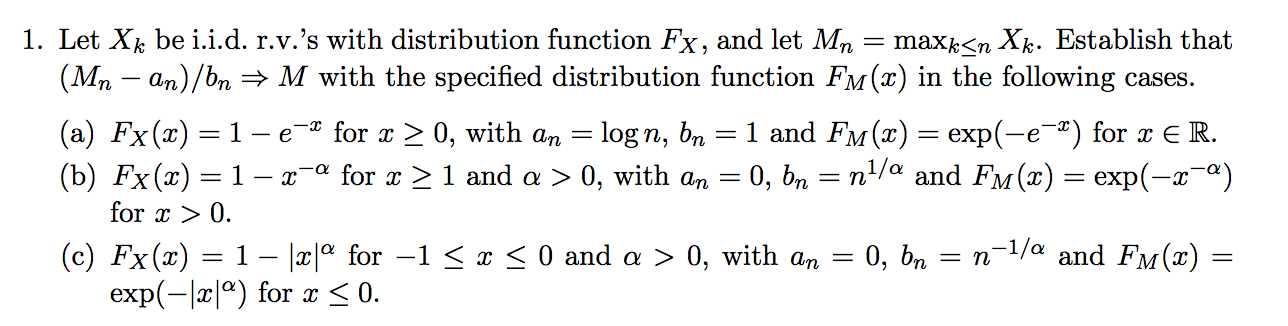
\includegraphics[width=0.7\textwidth]{prob-e5-p1.png}
\end{figure}
\end{question}
\begin{solution} \hfill \\
By i.i.d. assumption on $\{X_k\}$, 
\eQnb 
F_{\frac{M_n - a_n}{b_n}}(x) &=& 
\mathbb{P}(\dfrac{M_n - a_n}{b_n} \leq x) = \mathbb{P}(M_n \leq a_n + b_n x) 
= \mathbb{P}(\max_{k \leq n} X_k \leq a_n + b_n x )  \notag \\
&=& \mathbb{P}(\bigcap_{k \leq n} X_k \leq a_n + b_n x) 
= \prod_{k \leq n} \mathbb{P}(X_k \leq a_n + b_n x) = (F_{X}(a_n + b_n x))^n
\label{eq:1}
\eQne
for each $n \geq 1$ and $x \in \mathbb{R}$.

\bigskip

\textbf{(a)} Let $x \in \mathbb{R}$. Substituting the givens to \eqref{eq:1}, 
\eQb
F_{\frac{M_n - a_n}{b_n}}(x) &=& 
F_{X}(a_n + b_n x)^n = 
(1-e^{-\log(n) - x})^n = (1-\dfrac{-e^x}{n}))^n
\eQe
for all sufficiently large $n \in \mathbb{N}$.  
Taking the limit as $n \to \infty$ gives 
\eQb
\lim_{n \to \infty} F_{\frac{M_n - a_n}{b_n}}(x) = \exp(-e^{-x}) = F_M(x). 
\eQe
Therefore, $\dfrac{(M_n - a_n)}{b_n}$ converges in distribution to $M$.

\bigskip

\textbf{(b)} Let $x > 0$. Substituting the givens to \eqref{eq:1},
\eQb
F_{\frac{M_n - a_n}{b_n}}(x) &=& 
F_{X}(a_n + b_n x)^n = 
(1-(n^{\frac{1}{\alpha}}x)^{-\alpha})^n = (1-\dfrac{x^{-\alpha}}{n}))^n 
\eQe
for all sufficiently large $n \in \mathbb{N}$. Taking the limit as $n \to \infty$
gives
\eQb
\lim_{n \to \infty} F_{\frac{M_n - a_n}{b_n}}(x) &=& \exp(-x^{-\alpha}) = F_{M}(x).
\eQe
Let $x \leq 0$. Then 
\eQb
a_n + b_n x &=&  n^{\frac{1}{\alpha}}x \leq 0 
\eQe
and hence
\eQb
F_{\frac{M_n - a_n}{b_n}}(x) &=& (F_X(a_n + b_n x))^n = 0 
\eQe
for each $n \geq 1$. Since $F_{M}(x) = 0$ on for $x \leq 0$, we have shown that
\eQb
F_{\frac{(M_n - a_n)}{b_n}}(x) &\to& F_{M}(x)   
\eQe
for all $x \in \mathbb{R}$, and hence $\dfrac{M_n - a_n}{b_n}$ converges in
distribution to $M$. 

\bigskip

\textbf{(c)} Let $x < 0$. Then
\eQb
F_{\frac{M_n - a_n}{b_n}}(x) &=& (1 - |n^{-\frac{1}{\alpha}}x|^{\alpha})^n 
= (1 - \dfrac{|x|^{\alpha}}{n})^n
\eQe 
for all sufficiently large $n \in \mathbb{N}$. Taking the limit as $n \to \infty$
gives
\eQb
\lim_{n \to \infty} F_{\frac{M_n - a_n}{b_n}}(x) = \exp(-|x|^{\alpha}) = F_M(x).
\eQe 
Let $x \geq 0$. Then,
\eQb
a_n + b_n x = n^{-\frac{1}{\alpha}} x \geq 0
\eQe
and hence
\eQb
F_{\frac{m_n - a_n}{b_n}}(x) &=&  (F_X(n^{-\frac{1}{\alpha}}x))^n = 1
\eQe
for each $n \geq 1$. Since $F_M(x) = 1$ for all $x \geq 0$, we have shown that
\eQb
F_{\frac{(M_n - a_n)}{b_n}}(x) &\to& F_{M}(x)   
\eQe 
for all $x \in \mathbb{R}$ and hence $\dfrac{M_n - a_n}{b_n}$ converges in distribution
to $M$. 

\hfill $\qed$ 
\end{solution}

\newpage

\begin{question}[2]
\hfill
\begin{figure}[h!]
  \centering
    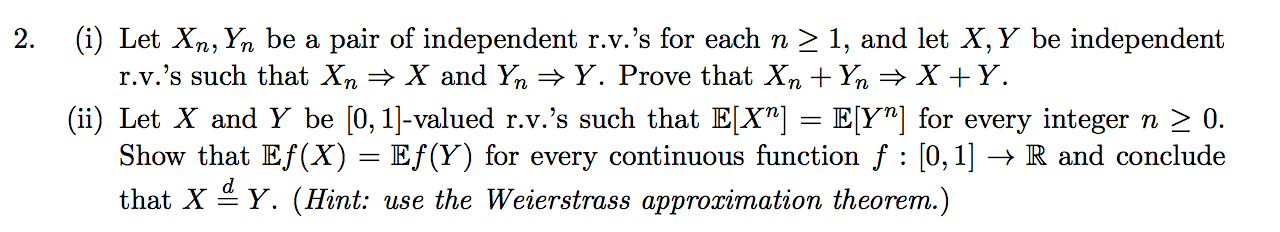
\includegraphics[width=0.7\textwidth]{prob-e5-p2.png}
\end{figure}
\end{question}
\begin{solution} \hfill \\
\textbf{(i)} Fix $t \in \mathbb{R}$. By independence, 
\eQb
\phi_{X_n + Y_n}(t) &=& \phi_{X_n}(t) \phi_{Y_n}(t) 
\eQe
and
\eQb
\phi_{X+Y}(t) &=& \phi_{X}(t)\phi_{Y}(t) 
\eQe
for each $n \geq 1$. By Levy-continuity theorem,
\eQb
\phi_{X_n}(t) \to \phi_{X}(t) \>\>\> \text{and} \>\>\> 
\phi_{Y_n}(t) \to \phi_{Y}(t)
\eQe
so 
\eQb
\lim_{n \to \infty} \phi_{X_n + Y_n}(t) &=& 
\lim_{n \to \infty} \phi_{X_n}(t) \phi_{Y_n}(t) = \phi_{X}(t) \phi_{Y}(t) = \phi_{X
+ Y}(t).
\eQe 
Therefore, $\{\phi_{X_n + Y_n} \}$ converges pointwise everywhere to $\phi_{X+Y}$,
so again by Levy-continuity theorem, we have $X_n + Y_n$ converges
in distribution to $X+Y$. 

\bigskip

\textbf{(ii)} As $X,Y$ are $[0,1]$-value random variables, by a change of variable,
\eQb
\int_{0}^{1} t^n \mu_X(dt) = \mathbb{E}[X^n] &=& 
\mathbb{E}[Y^n] = \int_{0}^{1} t^n \mu_Y(dt)
\eQe
for each $n \geq 1$. By linearity of integral, 
\eQb
\int_{0}^{1} p(t) \mu_X(dt) &=& \int_{0}^{1} p(t) \mu_Y(dt) \>\>\>\>\>\> (1)
\eQe
for any polynomial $p$ defined on $[0,1]$. Now, fix $\epsilon > 0$,
and by Weierstrass approximation theorem, choose a polynomial $p_0$ such that 
\eQb
||f - p_0||_{\sup} < \epsilon. 
\eQe
Then, by a change of variable and $(1)$,
\eQb
|\mathbb{E}[f(X)] - \mathbb{E}[f(Y)]| &=& 
|\int_{0}^{1} f(t) \mu_X(dt) - \int_{0}^{1} f(t) \mu_Y(dt)| \\
&=& |\int_{0}^{1} f(t) - p_0(t) \mu_X(dt) - \int_{0}^{1} f(t) - p_0(t) 
\mu_Y(dt)| \\
&\leq& \int_{0}^{1} |f(t) - p_0(t)| \mu_X(dt) + \int_{0}^{1} |f(t) - p_0(t)|
\mu_Y(dt) < 2\epsilon. 
\eQe
Since $\epsilon > 0$ was arbitrary, we have shown that $\mathbb{E}[f(X)] = 
\mathbb{E}[f(Y)]$ for any $f$ continuous and defined on $[0,1]$. Since $e^{ist}$
is continuous on $[0,1]$ for any fixed $s \in \mathbb{R}$, 
\eQb
\phi_{X}(s) &=& 
\mathbb{E}[e^{isX}] = \int_{0}^{1} e^{ist} \mu_X(dt) = \int_{0}^{1} e^{ist} 
\mu_Y(dt) = \mathbb{E}[e^{isY}] = \phi_{Y}(s)
\eQe 
for any $s \in \mathbb{R}$. Now, by Fourier Uniqueness, we have that $X = Y$
in distribution. \hfill $\qed$


\end{solution}

\newpage

\begin{question}[3]
\hfill
\begin{figure}[h!]
  \centering
    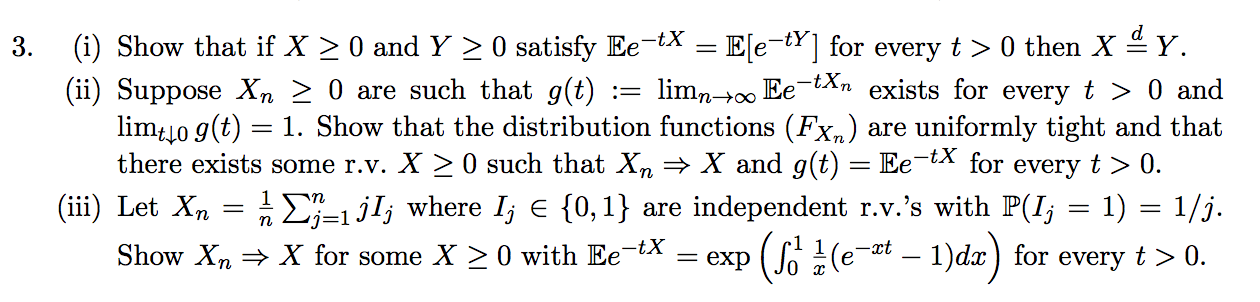
\includegraphics[width=0.7\textwidth]{prob-e5-p3.png}
\end{figure}
\end{question}
\begin{solution} \hfill \\
\textbf{(i)}
Observe that $e^{-X}$ and $e^{-Y}$ are $[0,1]$-valued random variables. Furthermore,
\eQb
\mathbb{E}[(e^{-X})^n] &=& \mathbb{E}[e^{-nx}] = \mathbb{E}[e^{-nY}] = 
\mathbb{E}[(e^{-Y})^n] 
\eQe 
for each $n \in \mathbb{N}$. Hence, by the problem $2-(ii)$, 
\eQb
e^{-X} \eqD e^{-Y}.
\eQe

\bigskip

\textbf{(ii)}

\textbf{(iii)}

\end{solution}

\newpage

\begin{question}[4]
\hfill
\begin{figure}[h!]
  \centering
    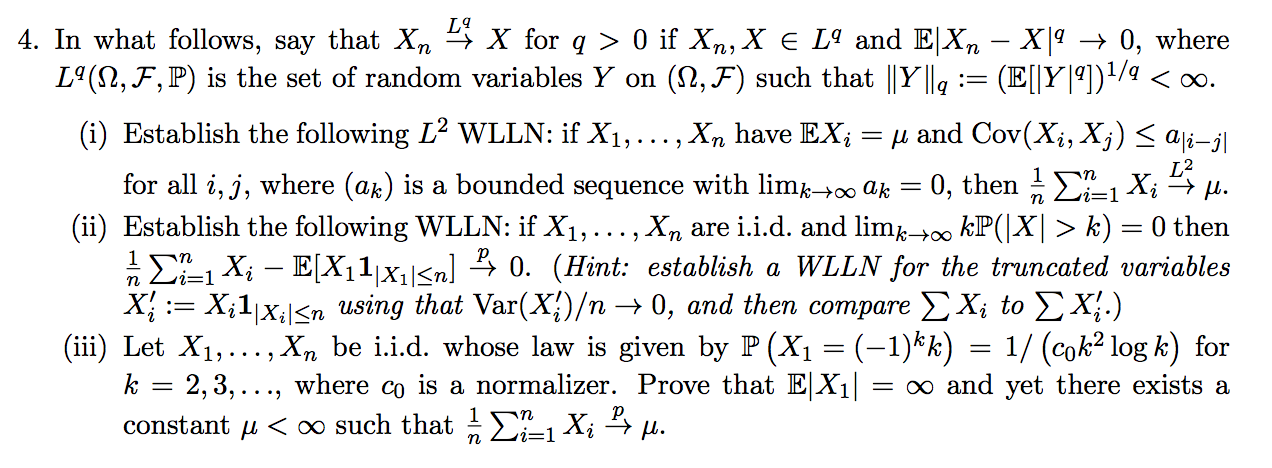
\includegraphics[width=0.7\textwidth]{prob-e5-p4.png}
\end{figure}
\end{question}
\begin{solution} \hfill \\
\end{solution}
\end{document}
